\documentclass[../main.tex]{subfiles}
\begin{document}
\chapter{Stato dell'arte}

In questo capitolo verrà presentato lo stato dell'arte per le soluzioni di analisi ed individuazione di minacce ai sistemi informatici. Si procede col fornire un'introduzione preliminare sulle tipologie di attacco affrontate in questa tesi.

\section{Malware}
Il termine malware è una combinazione delle parole \textit{malicious} e \textit{software}. Con questo termine si identificano tutti quei programmi software progettati per danneggiare o effettuare azioni illecite su un sistema informatico. \cite{MalwareDef}

Gli obiettivi che può avere un malware sono molteplici e sono in continua evoluzione. Il malware, a seconda dello scopo per cui è stato creato e alle sue caratteristiche, viene classificato nei seguenti modi:

\begin{verse}
				\textbf{Virus} Prendono il nome dai virus in campo biologico e si comportano in modo analogo, sono programmi che si replicano sul computer che hanno infettato e si predispongono ad infettare nuovi computer mediante mezzi di trasmissione quali email e chiavette USB. \cite{VirusDef}
\end{verse}

\begin{verse}
				\textbf{Spyware} Il termine Spyware è una combinazione delle parole \textit{Spy} e \textit{Software}. È un software che viene installato sul computer della vittima a sua insaputa e che raccoglie informazioni. 
				Uno spyware è oggetto di controversia perchè può essere utilizzato negli ambienti lavorativi per controllare le ricerche dei dipendenti o per controllare l'attività dei propri figli su internet. Anche se utilizzato per scopi più innocui può comunque violare la privacy dell'utente. \cite{Spyware2} \newline
				Usi più scorretti di programmi spyware prevedono di tracciare la cronologia internet di un utente per inviare pubblicità mirata, accedere alle password degli account in uso sul computer infetto e/o alle informazioni bancarie. Le informazioni raccolte attraverso l'uso di spyware possono essere utilizzate in vari modi, l'uso più frequente e più remunerativo ad oggi è quello di rivendere tali informazioni a dei terzi. \cite{Spyware1}
\end{verse}

\begin{verse}
				\textbf{Backdoor} Tradotto letteralmente come \textit{porta sul retro}, è un metodo utilizzato per avere un accesso privilegiato e spesso segreto che aggira il sistema di autenticazione previsto. Lo scopo di una backdoor è quello di permettere una connessione in remoto al computer vittima per prenderne il controllo.				
\end{verse}

\begin{verse}
				\textbf{Trojan} Il cavallo di Troia fu una macchina da guerra che, secondo la leggenda, fu usata dai greci per espugnare la città di Troia. Questo termine è entrato nel linguaggio comune per indicare uno stratagemma con cui penetrare le difese. Nell'ambito dei malware il trojan è un software che si nasconde all'interno di un altro programma all'apparenza innocuo e che, se eseguito, esegue anche il codice del trojan \cite{TrojanDef}.
				Oggi col termine trojan ci si riferisce principalmente ai malware ad accesso remoto. Spesso vengono utilizzati per installare backdoor sui sistemi bersaglio. \cite{TrojanPurpose}
\end{verse}

I malware erano inizialmente usati per compiere azioni dolose sia da hacker malintenzionati che dai governi per sottrarre informazioni personali, inviare spam e commettere frodi. \cite{ScopoMalware} \cite{MalwareRevolution}

L'evoluzione e lo sviluppo di internet hanno portato ad un incremento degli utenti connessi sempre maggiore. Questa crescita di internet ha spostato l'obiettivo dei malware che vengono usati sempre di meno per compiere azioni dolose. Fin dal 2003 la maggior parte dei malware sono stati creati per prendere il controllo dei computer dell'utente vittima per scopi illeciti \cite{MalwareRevolution}. Solitamente, le macchine infette vengono impiegate per l'invio di email di spam o per effettuare attacchi distribuiti Denial of Service (DDoS).


\section{Botnet}
Nella sua forma più semplice una Botnet è un gruppo di computer che sono stati infettati da un malware che consente ad un attaccante, detto anche \textit{botmaster}, di avere il controllo sulle macchine infettate. Le Botnet sono usate dal botmaster per compiere operazioni illecite ad insaputa della vittima. Una volta infetto, il computer della vittima prende il nome di \textit{zombie} (o, più semplicemente, "bot"). \cite{Botnet} \newline
Per aggiungere un computer ad una botnet si infetta il computer vittima con un malware che installa una backdoor in grado di consentire al botmaster di avere accesso remoto al computer infettato dal malware. Infettando molteplici host, il botmaster avrà così accesso ad un sistema gigantesco di computer zombie pronti ad essere attivati ed eseguire i suoi comandi. Le botnet rilevate e studiate nella letteratura dimostrano come questi sistemi possano arrivare a contenere anche milioni di computer infetti. \cite{Botnet}

I componenti di una botnet sono i seguenti:

\begin{verse}
				\textbf{Botmaster} Il botmaster rappresenta l'utente (o gli utenti) che detiene il il controllo remoto dell'intera botnet. La macchina utilizzata dal botmaster per comunicare con i vari bot viene tipicamente definita come \textit{Command and Control} (C\&C). I comandi (e le eventuali risposte) vengono inviati utilizzando protocolli e canali specifici, atti a minimizzare le possibilità di identificazione.
\end{verse}

\begin{verse}
				\textbf{Control protocol} Il protocollo utilizzato dal master per comunicare con i computer zombie.
\end{verse}

\begin{verse}
				\textbf{Computer zombie} Computer connesso ad internet che è stato infettato attraverso dei virus o trojan e che può essere utilizzato in modo remoto. 
\end{verse}

Nella figura~\ref{fig:architetturaBotnet} viene rappresentato una possibile architettura di una botnet, in cui il botmaster controlla in modo remoto i computer zombie attraverso dei server C\&C.
\begin{figure}[H]
				\centering
				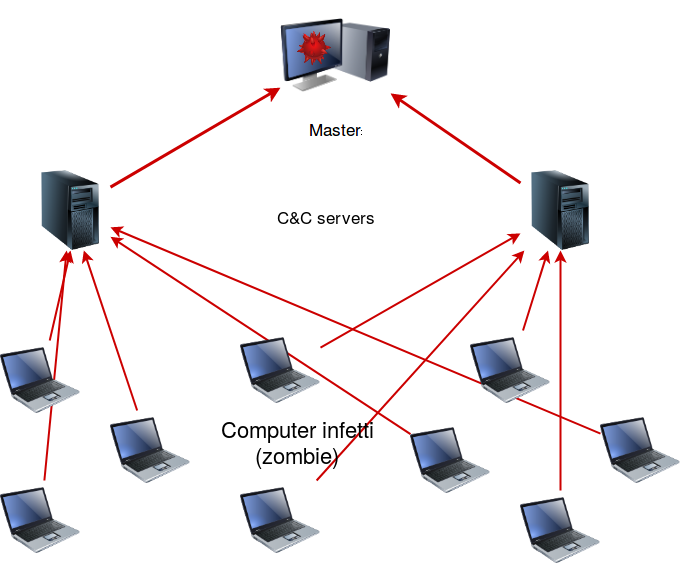
\includegraphics[scale=0.4]{botnet.png}
				\caption{Esempio architettura botnet}
				\label{fig:architetturaBotnet}
\end{figure}

I principali attacchi informatici effettuati attraverso l'utilizzo delle botnet sono vari: possono essere spam~\cite{botnetspam}, DDoS~\cite{ddosbotnet}, click fraud~\cite{clickfraudbotnet}, phishing~\cite{phishingbotnet} e bitcoin mining~\cite{bitcoinbotnet} per citarne alcuni. 

\begin{verse}
				\textbf{Spam} È l'invio tramite posta elettronica di messaggi contenenti truffe o pubblicità. Può essere di tipo \textit{orizzontale}, in cui si inviano più messaggi a molti utenti, o \textit{verticale}, in cui si puntano bersagli specifici con email mirate. Lo spam spesso confluisce nel phishing.
\end{verse}

\begin{verse}
				\textbf{Phishing} Con l'aumento di transazioni effettuate su internet il phishing è diventato sempre più comune \cite{phishing}. Il phishing è un tipo di truffa utilizzato per ottenere informazioni da utenti non esperti attraverso l'impersonazione di fonti attendibili \cite{phishingdef}.
\end{verse}

\begin{verse}
				\textbf{DDoS} Acronimo di Distributed Denial of Service, è un tipo di attacco in cui si mira a far esaurire le risorse di un sistema informatico affinchè non riesca più a fornire un servizio in maniera ottimale. Per fare ciò si inviano moltissime richieste al sistema in un breve periodo di tempo utilizzando i computer zombie. L'obiettivo è saturare la risorse disponibili (come la banda o la CPU), causando rallentamenti o il blocco completo del sistema.
\end{verse}

\begin{verse}
				\textbf{Click fraud} Questo tipo di frode si verifica sulla pubblicità su internet di tipo pay per click. Questo tipo di pubblicità genera quantità di denaro in base al numero di click effettuati sull'annuncio pubblicitario. Le botnet sfruttano questo tipo di pubblicità utilizzando computer zombie per cliccare in massa gli annunci pubblicitari.
\end{verse}

\begin{verse}
				\textbf{Bitcoin mining} I bitcoin~\cite{bitcoindef} vengono creati risolvendo operazioni matematiche complesse. Una botnet può utilizzare i computer zombie come unità di calcolo a cui far eseguire queste computazioni.
\end{verse}

\section{Botnet Detection}
Le botnet sono diventate il metodo preferito per lanciare attacchi su internet. Rappresentano una seria minaccia poichè possono inviare attacchi in modo coordinato e istantaneo da numerosi bot \cite{botnetdetection}. È stimato che ci sono milioni di bot attivi internet ogni giorno, di conseguenza è possibile identificare con le botnet una delle minacce più critiche per le organizzazioni moderne \cite{botnetdetection}.

Le botnet sono difficili da individuare dal momento che l'host autore dell'attacco non è visibile direttamente dalla vittima perchè nascosto da un layer di zombie. Un esempio di attacco è rappresentato in Figura~\ref{fig:zombieLayer}: il computer vittima non vede un attacco unico, ma un insieme di attacchi da una moltitudine di computer diversi che nascondono il botmaster.

\begin{figure}[H]
				\centering
				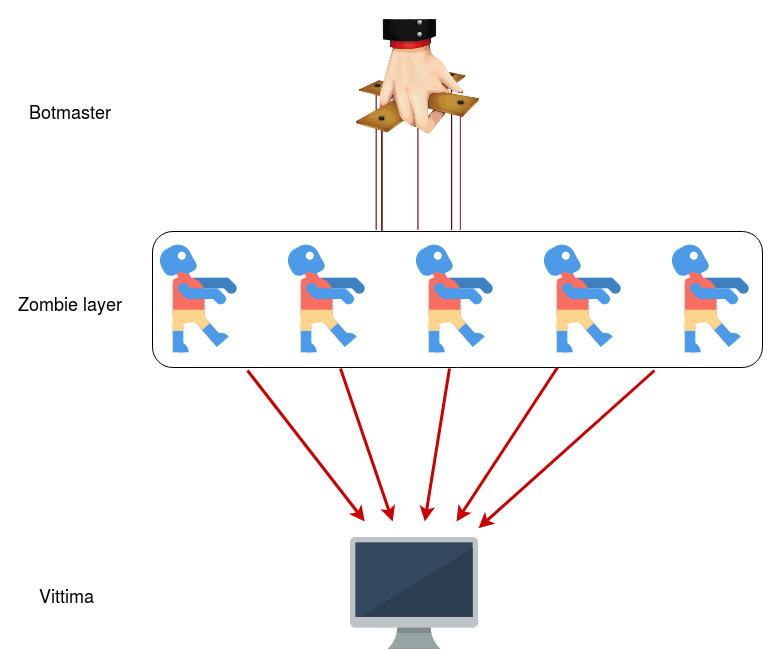
\includegraphics[scale=0.36]{zombielayer.png}
				\caption{Zombie layer}
				\label{fig:zombieLayer}
\end{figure}

Esistono in letteratura diversi metodi per la rilevazione delle botnet. Ad esempio, gli autori di~\cite{netflowbotnetdetection} utilizzano tecniche di clustering dei network flow per rilevare il traffico di rete prodotto dalle botnet, ma ottenendo un consistente quantitativo di falsi positivi. L'approccio descritto in~\cite{signaturebotnetdetection} è orientato al rilevamento delle botnet tramite l'utilizzo di signature, di fatto impedendo di identificare le botnet di nuova generazione di cui non si conoscono le caratteristiche. Esistono anche numerosi metodi basati sul data mining~\cite{dataminingbotnetdetection}, che sebbene siano teoricamente in grado di individuare nuove botnet, hanno la tendenza ad essere molto imprecisi. Un altro articolo~\cite{dnsbotnetdetection} presenta un elenco di metodi per il rilevamento delle botnet basato sui DNS; tuttavia non tutte le botnet fanno uso del DNS per comunicare con il rispettivo CnC server~\cite{brown2010resilient}. Infine, si segnalano gli approcci basati sugli honeypot~\cite{honeypotbotnetdetection}, che possono essere utili in caso di attaccanti poco esperti, ma che sono facilmente aggirabili in caso di avversari più competenti. In questa tesi ci si è focalizzato su tecniche basate sull'analisi dei modelli comportamentali.


\section{Intrusion Detection System}
In questa sezione verranno presentati i meccanismi utilizzati per identificare accessi non autorizzati ai sistemi informatici, che trovano anche impiego come strumenti per la rilevazione di botnet \cite{botnetdetection}.

Un'intrusione si verifica quando un aggressore tenta di entrare o interrompere le normali operazioni di un sistema informativo\cite{idsbook}. Esistono varie classi di intrusione che vanno rilevate: si possono verificare situazioni in cui un utente ruba una password, utenti legittimi che abusano dei loro privilegi o hacker che usano script trovati in rete per attaccare il sistema.

I sistemi di rilevamento delle intrusioni sono gli "allarmi antifurto" del campo della sicurezza informatica. L'obiettivo è difendere un sistema attraverso la segnalazione di allarmi, che vengono emessi ogni volta che viene rilevata un'attività sospetta \cite{IDS}. Tali sistemi prendono il nome di \textit{Intrusion Detection System} (IDS). Un IDS è un dispositivo software o hardware utilizzato per identificare intrusioni a singoli host o reti locali.

\subsection{Tipi di IDS}
Gli IDS possono essere di due tipi in base al target su cui vengono applicati: possono essere basati su rete o su host.
\begin{verse}
				\textbf{Host-Based IDS} Un IDS basato su host, detto HIDS, risiede su un particolare computer o server e monitora l'attività solo su quel sistema.
\end{verse}

\begin{verse}
				\textbf{Network-Based IDS} Un IDS basato sulla rete, detto NIDS, è installato su un computer o dispositivo collegato ad un segmento della rete e ne monitora il traffico alla ricerca di indicazioni di attacchi. Un IDS basato su rete può rilevare molti più attacchi rispetto ad un IDS basato su host, ma richiede una configurazione e manutenzione più complessa.
\end{verse}

Un IDS è composto da quattro componenti \cite{idsbook}:

\begin{itemize}
				\item \textbf{Sensori}, sono utilizzati per ricevere informazioni dalla rete o dai computer.

				\item \textbf{Console}, utilizzata per monitorare lo stato della rete e dei computer.

				\item \textbf{Motore}, analizza i dati prelevati dai sensori e provvede a individuare eventuali falle nella sicurezza.

				\item \textbf{Database}, memorizza le regole utilizzate per identificare violazioni di sicurezza.
\end{itemize}

L'immagine ~\ref{fig:esempioIds} descrive i componenti di un NIDS. I pacchetti in entrata e uscita dalla rete sono ricevuti da un sensore che raccoglie il traffico dati, successivamente il motore analizza i dati prelevati dai sensori con le regole presenti nel database.

\begin{figure}[H]
				\centering
				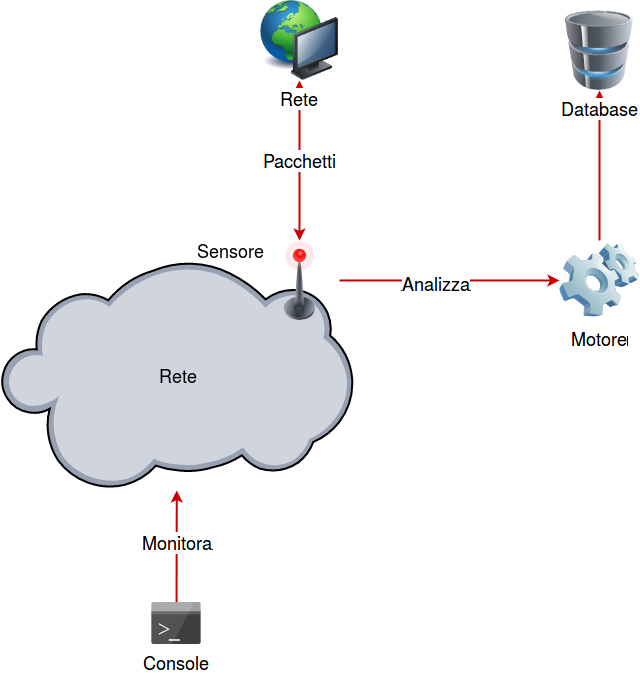
\includegraphics[scale=0.4]{IDS.png}
				\caption{Esempio di un IDS}
				\label{fig:esempioIds}
\end{figure}

Un'attuale estensione degli IDS sono gli Intrusion Prevention Systems, detti IPS. Tali strumenti, unitamente alla rilevazione di intrusioni, possono impedire l'esecuzione di azioni dannose per il sistema monitorato. Gli IPS usano diverse tecniche di risposte attive, che possono essere suddivise nei seguenti gruppi \cite{IPS}:

\begin{itemize}
				\item \textbf{terminare} la connessione internet o la sessione utente che sta eseguendo l'attacco
				\item \textbf{bloccare} l'accesso all'obiettivo e agli obiettivi simili all'utente o indirizzo IP che sta tentando un'intrusione
				\item \textbf{cambiare} l'ambiente di sicurezza modificando la configurazione di altri controlli di sicurezza per interrompere l'attacco, come la riconfigurazione delle regole di un firewall. Alcuni IPS possono anche applicare della patch di sicurezza a degli host se l'IPS rileva che l'host presenta delle vulnerabilità.
\end{itemize}

Poiché i due sistemi coesistono spesso, il termine combinato Intrusion Detection and Prevention System (IDPS) viene generalmente utilizzato per descrivere le attuali tecnologie anti-intrusione \cite{IPS}.


\subsection{Perchè usare IDS}
Dispositivi di tipo IDS sono utili per le difese di sistemi informatici per molteplici ragioni:
\begin{itemize}
				\item \textbf{defense in depth}, l'utilizzo di un dispositivo IDS unito a firewall~\cite{idswithfirewall}, controlli di accesso e autenticazione~\cite{idswithacl}, e antivirus~\cite{idswithav} permette la realizzazione di un meccanismo di protezione multi-livello 
				\item \textbf{documentazione}, i dati acquisiti sono utili anche per il miglioramento continuo della qualità. Gli IDS raccolgono costantemente informazioni sugli attacchi che hanno compromesso con successo gli strati esterni dei controlli di sicurezza, per esempio di un firewall. Queste informazioni possono essere utilizzate per identificare e riparare le vulnerabilità esposte dagli attacchi, di fatto aiutando l'organizzazione ad accelerare il processo di risposta agli incidenti e ad apportare miglioramenti continui.
Inoltre, sebbene un IDS non sia in grado di assicurare la prevenzione completa delle intrusioni, è comunque in grado di assistere nella revisione fornendo informazioni su come si è verificato l'attacco, assuieme ai dettagli sulle operazioni compiute dall'intruso. Gli IDS possono anche essere utilizzati in ambito forense, risultando utili anche per motivi legali \cite{IPS}
				\item \textbf{insider threat}, gli attacchi non sempre vengono effettuati da un attaccante esterno alla rete: spesso infatti sono gli utenti interni all'organizzazione che compiono azioni illegittime tentando di compromettere la rete dall'interno. Un IDS è in grado di segnalare anche questo tipo di "intrusioni"~\cite{IPS}
\end{itemize}

Si segnala anche l'importante funzione di deterrente svolta dalla presenza di un IDS. Se gli utenti esterni e interni sanno che un'organizzazione utilizza un sistema di rilevamento e prevenzione delle intrusioni, saranno meno propensi ad effettuare azioni malevole verso tale azienda\cite{IPS}.

\subsection{Metodi di rilevamento}

Gli IDS utilizzano vari metodi di rilevamento per monitorare e valutare il traffico di rete. I metodi principali sono \cite{IDS}:

\begin{verse}
				\textbf{Signature detection} Questo metodo di rilevamento delle intrusioni esamina il traffico di rete alla ricerca di pattern che corrispondono a firme note, ovvero pattern di attacco preconfigurati e predeterminati. Un vantaggio di questo approccio è che, avendo un modello con cui confrontare il comportamento che si sta osservando, il tasso di falsi positivi è molto ridotto. È inoltre veloce e semplice in quanto deve soltanto effettuare confronti con modelli illegali già noti.
				Uno svantaggio di questo approccio è che si possono verificare molti falsi negativi, cioè i comportamenti dannosi che non vengono segnalati. Ciò si verifica perchè questi sistemi sfruttano esclusivamente le regole per rilevare tipologie di attacco note; pertanto, in presenza di attacchi che presentano caratteristiche differenti dalle signature utilizzate per il confronto, non verrà segnalato alcun allarme. Ne segue che è quindi estremamente importante mantenere aggiornato il database delle signature con tutte le versioni più recenti di possibili comportamenti malevoli~\cite{snort}.
\end{verse}

\begin{verse}
				\textbf{Anomaly detection} Questo tipo di rilevamento si basa sull'idea che le azioni più sospette -- e quindi di maggiore interesse per un operatore della sicurezza -- sono quelle che presentano caratteristiche che deviano dalla normalità; pertanto, tali tecniche si basano sulla rilevazione di anomalie sistema analizzato. E' quindi necessario uno studio anticipato del sistema al fine di definirne il suo comportamento normale. In seguito, verrà poi stabilito quanto sia possibile discostarsi dal tipo di attività normale. 
				Il vantaggio principale di questo approccio consiste nella possibilità di rilevare anche attacchi non noti in precedenza, rendendoli efficaci contro attacchi che riescono ad eludere i sistemi basati su signature, e in alcuni casi anche contro attacchi di tipo zero-day~\cite{zerodaydef}.
				Gli svantaggi sono la difficoltà nella creazione dei modelli di "normalità"; e la tendenza di queste tecniche a generare un numero considerevole di falsi positivi~\cite{suricatadef}.
\end{verse}

\section{Machine learning}
Il machine learning rappresenta uno degli sviluppi più prolifici dell'intelligenza artificiale moderna \cite{compIntelligence}. L'enfasi del machine learning è sulla capacità del sistema di adattarsi o cambiare, in genere in risposta a qualche forma di esperienza fornita al sistema. Dopo l'apprendimento ci si aspetta che il sistema migliori le prestazioni future sullo stesso compito o lavori simili.

Negli ultimi anni il machine learning ha preso sempre più piede ed è ormai utilizzato quasi ovunque \cite{compIntelligence}. Alcuni esempi di applicazioni di machine learning nel mondo reale sono il controllo di robot autonomi in grado di navigare da soli, si pensi alle macchine con pilota automatico che stanno entrando in commercio negli ultimi anni come la Tesla di Elon Musk \cite{tesla}; il filtro dello spam nelle email \cite{spamemail}, il riconoscimento della calligrafia impiegato da software \textit{Optical Character Recognition} \cite{ocr}, il riconoscimento vocale degli assistenti presenti su dispositivi come Google Home \cite{googlehome}, Amazon Alexa \cite{amazonalexa} o Apple HomePod \cite{applehomepod}; il rilevamento dei volti nelle fotocamere digitali \cite{facialrecognition} e così via.
Per problemi come il riconoscimento vocale gli algoritmi basati sul machine learning superano tutti gli approcci che sono stati tentati fino ad oggi \cite{mldef}.

% In un contesto di machine learning si dice feature un dato in input che rappresenta una proprietà osservabile. Dalle feature, attraverso un paradigma di apprendimento, viene creato un modello. Si dice label un dato in output che corrisponde ad una feature in input. In base alla gestione delle features e delle labels si hanno differenti paradigmi di apprendimento. ****QUESTO PARAGRAFO E' ASSOLUTAMENTE INCOMPRENSIBILE ****

Generalmente esistono tre paradigmi di machine learning\cite{ai}.
\begin{verse}
				\textbf{Supervised learning} Questo paradigma prevede una fase di training in cui viene fornito un apposito dataset definito da una serie di features\footnote{In ambito di machine learning, si utilizza il termine \textit{feature} per indicare una proprietà misurabile di un determinato sample (dato). Ogni sample fornito in input ad un qualsiasi algoritmo di machine learning sarà quindi identificato da una serie di features.}, insieme alle corrispondenti label\footnote{Le labels vengono utilizzate per indicare cosa rappresenta un determinato sample}. L'obiettivo è ottenere un modello in grado di effettuare previsioni su samples non precedentemente noti, analizzandone le features e confrontandole con la conoscenza acquisita in fase di training.
\end{verse}

\begin{verse}
				\textbf{Unsupervised learning} Questo paradigma si differenzia dal Supervised Learning in quanto non richiede una fase di training con dataset labellati. Vengono forniti in input dei samples che consistono di sole features, ma non viene fornita alcuna label. L'obiettivo è scoprire nuove proprietà nei dati forniti in input attraverso l'ottimizzazione di un principio di apprendimento.
\end{verse}

\begin{verse}
				\textbf{Reinforced learning} Paradigma che si basa sul principio dell'\textit{esplorazione}. Osservando lo stato attuale dell'ambiente e analizzandone le feature, il modello compie un'azione che cambia lo stato dell'ambiente, ricevendo poi una valutazione positiva o negativa sull'azione compiuta. L'obiettivo è compiere una serie di azioni tali da massimizzare la valutazione ricevuta.
\end{verse}

\subsection{Supervised learning}
Al computer supervisionato vengono forniti dei dati chiamati \textit{training data}. Questi dati sono dei campioni, ognuno dei quali consiste in una serie di features insieme all'output desiderato.

In base al valore di output si distinguono due diversi problemi:

\begin{itemize}
				\item \textbf{Classificazione} Se il valore di output è discreto, ad esempio l'appartenenza o la non appartenenza ad una determinata classe.
				\item \textbf{Regressione} Se il valore dell'output è un valore reale continuo in un determinato range.
\end{itemize}

In entrambi i problemi si vuole trovare una funzione \textit{h}, che dato un input non conosciuto stima il valore dell'output. L'obiettivo dei problemi di supervised learning è quello di fare una predizione basata su proprietà conosciute apprese durante la fase di training.

La figura ~\ref{fig:supervisedLearning} descrive un problema di supervised learning, dove l'algoritmo di machine learning prende in input un insieme di esempi da cui impara una funzione che gli permette di fare previsioni.

\begin{figure}[H]
				\centering
				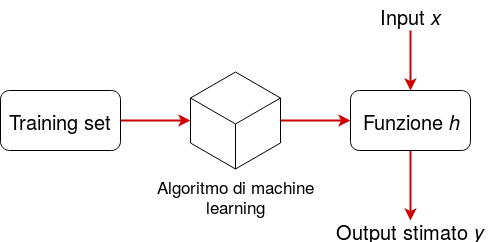
\includegraphics[scale=0.5]{apprendimentosupervisionato.png}
				\caption{Supervised learning}
				\label{fig:supervisedLearning}
\end{figure}

Un esempio di algoritmo supervised sono le reti neurali.
\subsubsection{Reti neurali}
Una rete neurale è un algoritmo che si ispira ai neuroni nel cervello umano. Ogni neurone è responabile della risoluzione di una parte molto piccola del problema, che nel complesso permette al cervello di risolvere problemi difficili. In modo simile una rete neurale è composta da cellule che lavorano insieme per produrre un risultato desiderato. La rete inizia con un input che attraversa i neuroni. Se un particolare neurone riceve abbastanza stimoli invia un messaggio a qualsiasi altro neurone a cui è collegato.

La figura~\ref{fig:retineurali} rappresenta una semplice neurone che controlla se una persona è viva. Controlla due input: il battito e il respiro. Se il neurone riceve uno stimolo da entrambi restituisce in output che la persone è viva.

\begin{figure}[H]
				\centering
				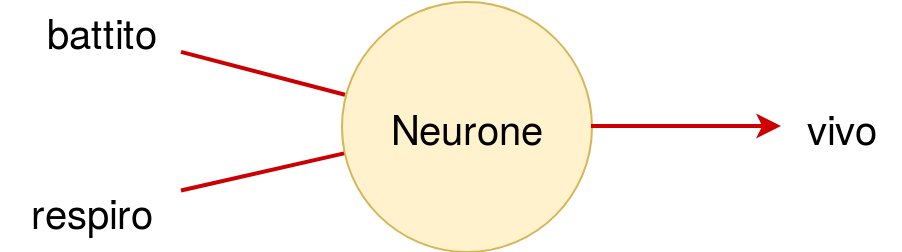
\includegraphics[scale=0.3]{retineurali.png}
				\caption{Esempio di neurone}
				\label{fig:retineurali}
\end{figure}

Questi algoritmi possono trovare applicazione in IDS~\cite{reteneuraleids}.

\subsubsection{Modelli probabilistici}
I metodi probabilistici sono fondamentali per il machine learning \cite{compIntelligence}. La funzione $h$, per stimare il valore dell'output, sceglie i parametri che massimizzano la probabilità dei dati che lega i valori degli input ai valori degli output.

\subsubsection{Modelli di Markov}
Le serie temporali e, più in generale le sequenze, sono una forma di dati strutturati che rappresenta un elenco di osservazioni per le quali è possibile definire un ordine completo, come ad esempio il tempo in una sequenza temporale.

Sia una sequenza di lunghezza $T$, $ { y } _ { n } = y _ { 1 } , \dots , y _ { T }$. Il termine ${y} _ {t}$ indica l'osservazione $t$-esima rispetto all'ordine totale. Siccome gli elementi che compongono la sequenza non sono indipendenti e identicamente distribuiti, la distribuzione congiunta di un modello probabilistico per $y$ è $P \left( Y _ { 1 } , \ldots , Y _ { T } \right)$.

Per osservazioni ${y} _ {t}$ a valore discreto la distribuzione congiunta cresce esponenzialmente con le dimensioni del dominio di osservazione. Per ridurre la parametrizzazione si usano le \textit{Catene di Markov}. Le Catene di Markov semplificano assumendo che un'osservazione che si verifica in una posizione $t$ della sequenza dipende solo da un numero limitato di predecessori rispetto all'ordine completo.
Ciò significa che in una serie temporale un'osservazione al tempo presente tiene conto soltanto di un numero limitato di osservazioni del passato.

Le Catene di Markov stanno alla base dei \textit{Modelli di Markov nascosti} (HMM).

\subsubsection{Catena di Markov}
Una Catena di Markov è un processo stocastico per sequenze. Presuppone che un'osservazione ${y} _ {t}$ a tempo $t$ dipenda solo da un insieme finito di predecessori $L \geq 1$. Il numero di predecessori $L$ che influenzano la nuova osservazione è detto ordine della Catena di Markov.

Una catena di Markov di ordine $L$ è una sequenza di variabili casuali $\mathbf { Y } = Y _ { 1 } , \ldots , Y _ { T }$ tali che $\forall t \in \{ 1 , \ldots , T \}$

\begin{center}
				\begin{math}
								P \left( Y _ { t } = y _ { t } | Y _ { 1 } , \ldots , Y _ { t - 1 } , Y _ { t + 1 } , \ldots , Y _ { T } \right) = P \left( Y _ { t } = y _ { t } | Y _ { t - L } , \ldots , Y _ { t - 1 } \right)
				\end{math}
\end{center}

\subsubsection{Modelli di Markov nascosti}
Le Catene di Markov modellano i dati sequenziali assumendo che gli elementi della sequenza siano generati da un processo stocastico completamente osservabile. Nella maggior parte dei sistemi reali l'unica informazione disponibile può essere il risultato del processo stocastico ad ogni osservazione ${y} _ {t}$ mentre lo stato del sistema rimane nascosto. 

\subsection{Unsupervised learning}
In questa categoria vengono forniti dei samples con relative feature in input, ma non viene fornita alcuna label. L'obiettivo di questi algoritmi è quello di trovare delle caratteristiche comuni nei dati forniti in input. Se si vogliono identificare dei raggruppamenti di elementi simili, è un problema di Clustering.


\begin{verse}
				\textbf{Clustering} È un tipico esempio di unsupervised learning in cui, dato un insieme di features senza labels, l'obiettivo è quello di individuare dei raggruppamenti, detti cluster, quanto più possibile coerenti. Un esempio di algoritmo di Clustering è il K-Means.
\end{verse}	

\subsubsection{K-Means}
L'algoritmo K-Means è uno degli algoritmi di clustering più conosciuti e più utilizzati. Permette di suddividere un insieme di oggetti in $K$ gruppi sulla base dei loro attributi.
Si assume che gli attributi degli oggetti possano essere rappresentati come vettori, e che quindi formino uno spazio vettoriale. Dal \textit{dataset} fornito vengono inizializzati $n$ punti detti centroidi per ogni cluster che è necessario identificare.

In figura ~\ref{fig:means1} vengono inizializzati due centroidi con una croce rossa e blu.

\begin{figure}[H]
				\centering
				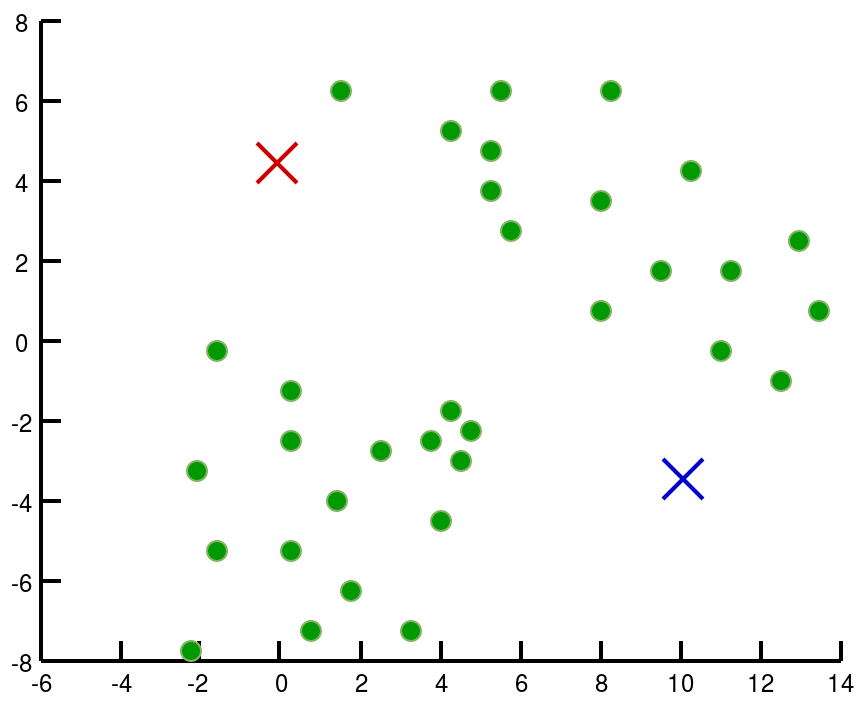
\includegraphics[scale=0.3]{k-means1.png}
				\caption{Algoritmo k-means - Inizializzazione}
				\label{fig:means1}
\end{figure}

L'algoritmo segue una procedura iterativa che ripete due passi, il primo è il passo di assegnazione ai cluster, mentre il secondo è il passo di spostamento dei centroidi.
Il primo passo di assegnazione ai cluster controlla la distanza di ogni punto del dataset dai centroidi e assegna ciascun punto al centroide che gli è più vicino. 
La figura ~\ref{fig:means2} rappresenta questo primo passo: i punti più vicini al centroide rosso sono stati colorati di rosso, mentre quelli più vicini al centroide blu sono stati colorati di blu.

\begin{figure}[H]
				\centering
				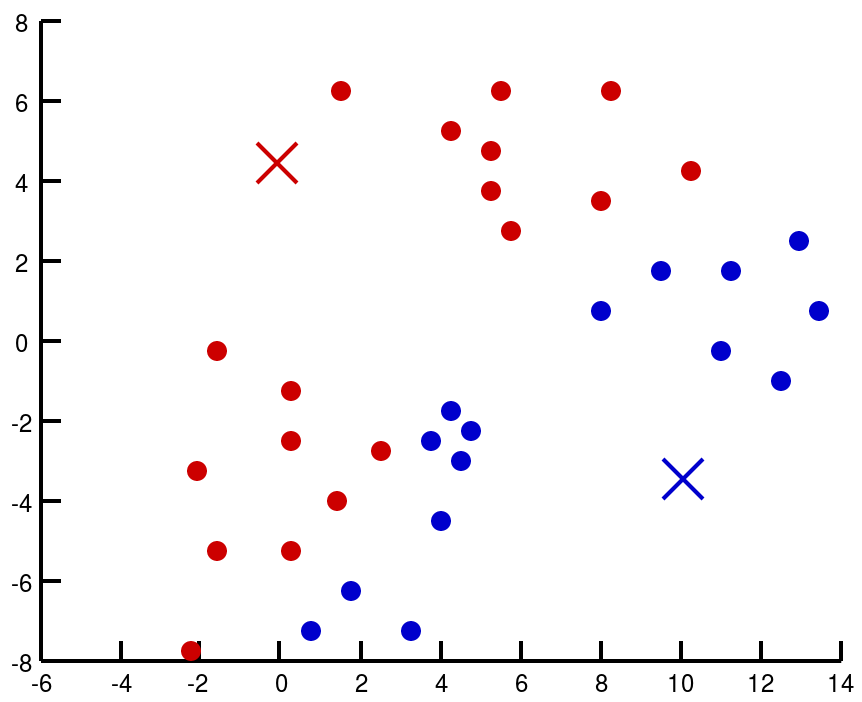
\includegraphics[scale=0.3]{k-means2.png}
				\caption{Algoritmo k-means - Passo 1}
				\label{fig:means2}
\end{figure}

Il secondo passo consiste nel calcolare la media di tutti i punti nel dataset che appartendono ad un cluster e muovere in quella posizione il centroide del cluster. Questo passo viene descritto in figura ~\ref{fig:means3}

\begin{figure}[H]
				\centering
				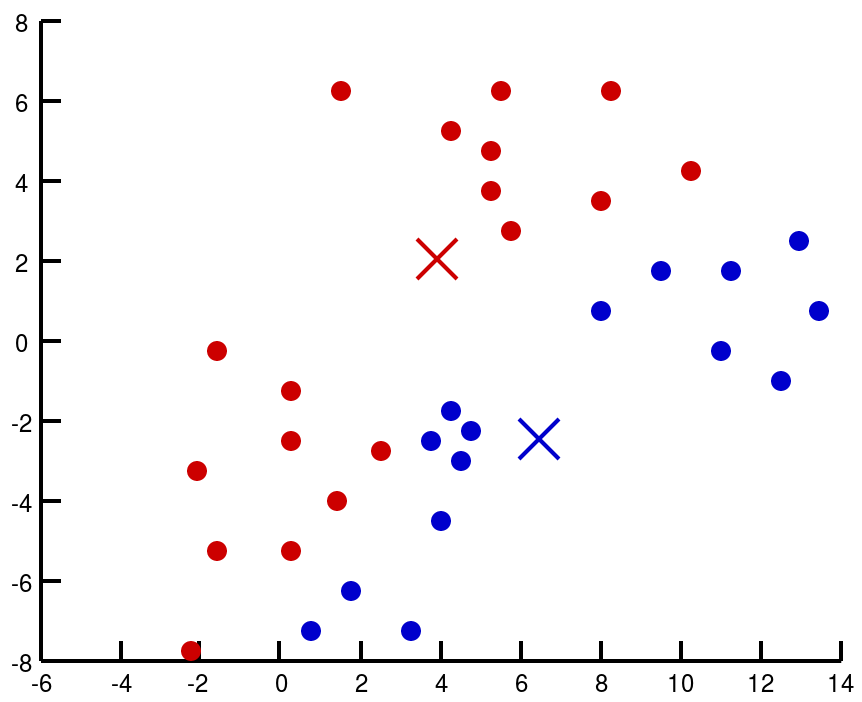
\includegraphics[scale=0.3]{k-means3.png}
				\caption{Algoritmo k-means - Passo 2}
				\label{fig:means3}
\end{figure}

L'algoritmo continua a ripetere questi due passi fino a quando i centroidi non si spostano più, il che significa che l'algoritmo ha raggiunto la convergenza e i due cluster sono stati individuati.

\begin{figure}[H]
				\centering
				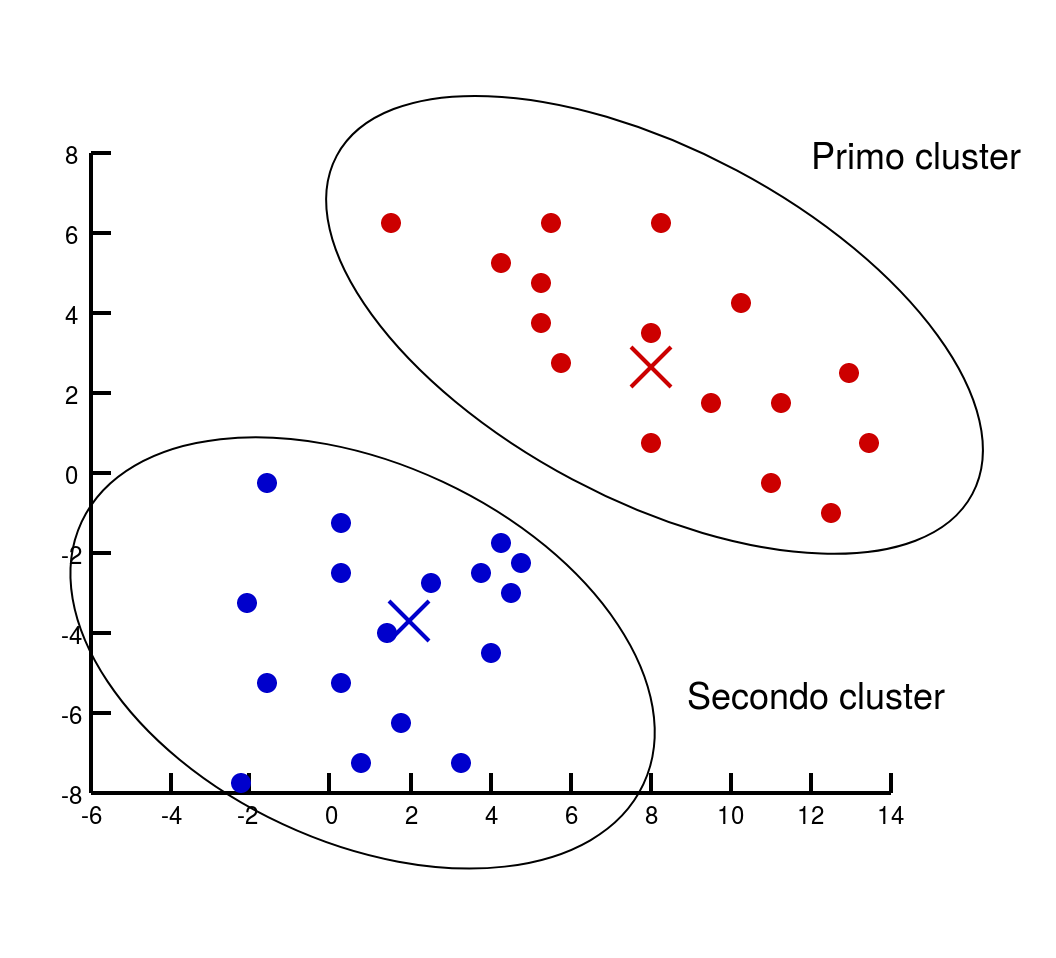
\includegraphics[scale=0.3]{k-means4.png}
				\caption{Algoritmo k-means - Convergenza}
\end{figure}

Algoritmi di clustering sono usati per fare botnet detection dagli IDS~\cite{netflowbotnetdetection}.

\subsection{Reinforced learning}
A differenza dell'unsupervised learning, il reinforced learning viene indirizzato dalla valutazione esterna. Inoltre a differenza del supervised learning in cui viene specificato l'output corrispondente ad un input, nel reinforced learning viene fornita solo una valutazione sull'azione compiuta.

In aggiunta, questo tipo di machine learning è caratterizzato da un processo dinamico in fasi discrete: ad ogni passo, osservando l'ambiente circostante e ottenendo qualche input, il computer compie un'azione e si sposta in un nuovo stato, venendo premiato o punito in base all'azione effettuata \cite{compIntelligence}.

\subsubsection{Processo decisionale di Markov}
Il reinforced learning è strettamente correlato con il processo decisionale di Markov \cite{compIntelligence}, che consiste in una serie di stati $s _ { 0 } , s _ { 1 } , \ldots , s _ { t } , s _ { t + 1 } , \ldots$. Allo stato ${ s } _ { t }$, un'azione $a _ { t } = \pi \left( s _ { t } \right)$ è selezionata da un insieme $A$ di azioni intraprese in funzione dello stato $\pi$, che fa muovere l'ambiente per raggiungere lo stato successivo $s _ { t  + 1}$ e la valutazione $v _ {t + 1}$ associata con la transizione $\left( s _ { t } , a _ { t } , s _ { t + 1 } \right)$ viene assegnata. L'obiettivo è ottenere la valutazione più alta possibile, cioè di massimizzare 

\begin{center}
				\begin{math}
								R = \sum _ { t = 0 } ^ { N - 1 } r _ { t + 1 }
				\end{math}
\end{center}

con $N$ istante di tempo in cui lo stato finale è raggiunto.



\end{document}
